\section{Original context study: method and primary comparisons}
\label{app:original-context-study}
This appendix preserves the original context-based protocol and its completed primary planning comparisons. In these original-study tables and figures, ShiftWM denotes Ours-1. The subsequent spatial variants use separate representations and development protocols.

\subsection{Problem and information access}
\label{sec:problem}
Let $x_t$ be hidden physical state, $a_t$ an executed action, $p$ a dynamics
setting, and $v$ an observation setting. Within a stationary segment,
\begin{equation}
 x_{t+1}=F_p(x_t,a_t,\epsilon_t),\qquad o_t=R_v(x_t,\eta_t).
 \label{eq:environment}
\end{equation}
The deployed agent receives images and actions, not $x_t,p,v$.
Training covers selected pairs $(v,p)$. Compositional testing holds out a
pair while retaining each factor individually in training; extrapolation
to new values is a separate evaluation. Appearance transforms preserve the
action coordinate system. Camera geometry changes and noninvertible
occlusion require different protocols.

An earlier support segment $S$ contains $H$ observations and $H-1$ actions;
later query images $Q$ are disjoint from support. At deployment, support
is real past history, and the controller receives a goal image. Imagined
futures never become evidence for context inference. Complete trajectory
families, including appearance-paired renders, stay within one data split.

\paragraph{Training supervision and fairness.}
A canonical render depicts the \emph{same physical state} under a reference
appearance; changing dynamics requires a new rollout. All trained controls
receive the same trajectories, canonical targets, training schedule, and
validation selection. ShiftWM additionally uses pairing identities for
context consistency. Shared versus unpaired contexts tests architecture;
unpaired contexts versus ShiftWM tests the extra consistency supervision.
A comparison against the frozen model alone cannot attribute a gain to
factorization.

\subsection{ShiftWM: observation and dynamics contexts}
\label{sec:method}
The visual encoder and projector $E_0$ are frozen. We train context networks,
adapters, the action encoder, predictor, and prediction projector offline.
Weights remain fixed online. Figure~\ref{fig:method} foregrounds the shared
observation calibration (A), corrected-transition dynamics inference (B), and
additional paired supervision (C); the LeWM backbone and CEM planner are
reused. Appendix~\ref{sec:implementation} gives
dimensions, initialization, and parameter counts.

\begin{figure}[t]
\centering
\resizebox{\linewidth}{!}{% Proposed components A/B and training-only pair constraints C.
% Real observed inputs and training representatives; features/paths remain schematic.
\begin{tikzpicture}[x=1cm,y=1cm,font=\sffamily\fontsize{8.5}{10}\selectfont,text=ink,
 flow/.style={-{Latex[length=2.9pt,width=2.2pt]},draw=ink!58,line width=.7pt,line cap=round,line join=round},
 obsflow/.style={flow,draw=obsblue,line width=.85pt},
 actflow/.style={flow,draw=dynorange,line width=.85pt},
 pair/.style={<->,>=Latex,dashed,line width=.85pt},
 shell/.style={draw=ink!22,fill=white,rounded corners=2pt,line width=.5pt,inner sep=0pt},
 badge/.style={circle,minimum size=.43cm,inner sep=0pt,text=white,font=\sffamily\bfseries\fontsize{8.5}{10}\selectfont},
 title/.style={font=\sffamily\bfseries\fontsize{9.5}{11}\selectfont},
 code/.style={circle,minimum size=.68cm,inner sep=0pt,line width=.8pt}]
\path[use as bounding box] (0,-.70) rectangle (14,11.30);
\node[title] at (2.06,10.96) {Observed inputs};
\node[badge,fill=obsblue] at (5.84,10.96) {A};
\node[title,anchor=west,text=obsblue] at (6.13,10.96) {Shared calibration};
\node[badge,fill=dynorange] at (10.08,10.96) {B};
\node[title,anchor=west,text=dynorange] at (10.36,10.96) {Dynamics inference};

% Deployment input examples. The entire support filmstrip owns the output port.
\node at (3.20,10.13) {Goal $o_g$};
\node[shell,minimum width=1.31cm,minimum height=1.31cm] (goal) at (3.20,9.13) {};
\node[inner sep=0pt] at (3.20,9.13) {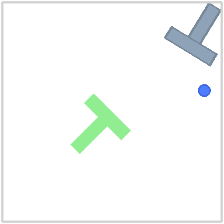
\includegraphics[width=1.20cm]{figures/assets/method_pusht_frame_7.png}};
\node at (2.06,8.15) {Observed history $o_S$};
\fill[ink!5,rounded corners=2pt] (.45,6.48) rectangle (3.90,7.87);
\node[shell,minimum width=3.55cm,minimum height=1.30cm] (history) at (2.08,7.23) {};
\foreach \idx/\xx in {0/.93,1/2.08,2/3.23}{
 \node[inner sep=0pt] at (\xx,7.23) {\includegraphics[width=1.10cm]{figures/assets/method_pusht_frame_\idx.png}};
}
\foreach \yy/\tag in {9.13/goal,7.23/history}{
 \node[shell,fill=ink!3,minimum width=.57cm,minimum height=.65cm] (enc\tag) at (4.42,\yy) {$E_0$};
 \node[inner sep=0pt] at (4.42,\yy+.52) {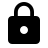
\includegraphics[width=.20cm]{figures/assets/material_lock.png}};
}
\draw[flow] (goal.east) -- (encgoal.west);
\draw[flow] (history.east) -- (enchistory.west);

% A: one visibly shared channel-wise affine map of goal and support features.
\fill[obsblue!12,rounded corners=3pt] (5.92,6.58) rectangle (8.33,9.74);
\draw[fill=obsblue!3,draw=obsblue!55,line width=.85pt,rounded corners=3pt]
 (5.85,6.64) rectangle (8.25,9.80);
\node[text=obsblue,font=\fontsize{15}{17}\selectfont] at (7.05,8.39) {$A_o$};
\node[text=obsblue] at (7.05,8.01) {scale + shift};
\foreach \yy/\offset in {9.13/0,7.23/.07}{
 \fill[white,rounded corners=1.3pt] (5.97,\yy-.38) rectangle (8.12,\yy+.38);
 \foreach \xin/\xout/\hh/\scale/\shift/\shade in {
  6.05/7.42/.18/1.08/.12/35,6.22/7.59/.44/.94/-.05/60,
  6.39/7.76/.30/1.06/.13/43,6.56/7.93/.53/.96/-.08/73}{
  \pgfmathsetmacro{\beforeHeight}{\hh-\offset}
  \pgfmathsetmacro{\afterHeight}{\scale*\beforeHeight+\shift}
  \fill[ink!\shade] (\xin,\yy-.27) rectangle ++(.115,\beforeHeight);
  \fill[obsblue!\shade] (\xout,\yy-.27) rectangle ++(.115,\afterHeight);
 }
 \node[text=obsblue,font=\fontsize{12}{14}\selectfont] at (7.05,\yy) {$\times\!+$};
}
\draw[flow] (encgoal.east) -- (5.85,9.13);
\draw[flow] (enchistory.east) -- (5.85,7.23);
\node at (5.14,9.42) {$u_g$};
\node at (5.14,7.53) {$u_S$};
\node[shell,draw=obsblue!55,fill=obsblue!4,minimum width=2.40cm,minimum height=.66cm]
 (obsinfer) at (7.05,6.09) {};
\node[text=obsblue] at (6.36,6.09) {$\mu,\sigma^2$};
\draw[obsflow] (6.88,6.09) -- (7.38,6.09);
\node[text=obsblue,font=\fontsize{12}{14}\selectfont] at (7.80,6.09) {$c_o$};
\draw[flow] (5.25,7.23) -- (5.25,6.09) -- (obsinfer.west);
\fill[ink!60] (5.25,7.23) circle[radius=.026];
\draw[obsflow] (obsinfer.north) -- (7.05,6.64);
\node[text=obsblue] at (7.05,10.25) {same $A_o$, same $c_o$};

% B: chronological corrected transitions and actual executed actions.
\node at (11.68,10.15) {Executed $a_S$};
\node[shell,draw=dynorange!35,fill=dynorange!3,minimum width=1.55cm,minimum height=.42cm]
 (executed) at (11.68,9.66) {};
\draw[actflow] (11.11,9.66) -- (11.48,9.66);
\draw[actflow] (11.86,9.57) -- (12.23,9.75);
\node[shell,draw=dynorange!60,fill=dynorange!3,minimum width=3.45cm,minimum height=1.32cm]
 (dyninfer) at (11.73,7.49) {};
\foreach \xx/\shade in {10.23/45,10.38/65,10.98/55,11.13/80}{
 \fill[obsblue!\shade] (\xx,7.00) rectangle ++(.10,.42);
}
\draw[obsflow] (10.61,7.22) -- (10.86,7.22);
\node[text=obsblue] at (10.75,7.81) {$z_t,\Delta z_t$};
\node[shell,draw=dynorange!45,minimum width=.72cm,minimum height=.48cm] (gru) at (12.00,7.23) {GRU};
\draw[flow] (11.35,7.23) -- (gru.west);
\node[text=dynorange,font=\fontsize{12}{14}\selectfont] (cd) at (13.02,7.23) {$c_d$};
\draw[actflow] (gru.east) -- (cd.west);
\draw[actflow] (executed.south) -- (11.68,8.85) -- (12.00,8.85) -- (gru.north);
\draw[obsflow] (8.25,7.23) -- (10.00,7.23);
\node[text=obsblue] at (8.91,7.53) {$z_S$};
\fill[obsblue] (8.78,7.23) circle[radius=.027];

% Conventional planning is quiet gray; each candidate yields latent futures.
\node[shell,fill=ink!3,minimum width=.76cm,minimum height=.73cm] (predictor) at (9.20,5.12) {$P$};
\node[shell,fill=dynorange!3,draw=dynorange!40,minimum width=1.11cm,minimum height=.73cm]
 (ad) at (10.85,5.12) {$A_d\circ E_a$};
\node[shell,fill=ink!2,minimum width=1.74cm,minimum height=.73cm] (candidates) at (12.65,5.12) {};
\foreach \xx in {12.15,12.65,13.15}{
 \draw[draw=ink!30,rounded corners=1pt] (\xx-.20,4.96) rectangle (\xx+.20,5.28);
 \draw[flow] (\xx-.13,5.12) -- (\xx+.13,5.12);
}
\node at (12.52,5.77) {candidates};
\node[text=ink!65] at (9.20,4.59) {LeWM};
\draw[obsflow] (8.78,7.23) -- (8.78,6.48) -- (9.20,6.48) -- (predictor.north);
\draw[actflow] (cd.south) -- (13.02,6.48) -- (10.85,6.48) -- (ad.north);
\draw[flow] (candidates.west) -- (ad.east);
\draw[flow] (ad.west) -- (predictor.east);

% Three schematic latent sequences. The outlined left token is terminal.
% No pixel predictions, measured candidate scores, or winning candidate implied.
\node[shell,fill=ink!1,minimum width=2.03cm,minimum height=1.29cm]
 (futures) at (7.50,4.99) {};
\node at (7.50,5.42) {Latent futures};
\foreach \yy/\shade in {5.06/40,4.80/55,4.54/70}{
 \foreach \xx/\step in {8.06/0,7.51/1,6.96/2}{
  \draw[draw=ink!35,fill=white,rounded corners=.4pt,line width=.45pt]
   (\xx-.16,\yy-.09) rectangle (\xx+.16,\yy+.09);
  \foreach \dx/\ht/\phase in {-.10/.07/0,-.025/.11/70,.05/.05/145}{
   \pgfmathsetmacro{\schematicHeight}{\ht+.025*sin(55*\step+\phase+\shade)}
   \fill[ink!\shade] (\xx+\dx,\yy-.055) rectangle ++(.04,\schematicHeight);
  }
 }
 \draw[flow,line width=.5pt,-{Latex[length=1.8pt,width=1.4pt]}] (7.88,\yy) -- (7.69,\yy);
 \draw[flow,line width=.5pt,-{Latex[length=1.8pt,width=1.4pt]}] (7.33,\yy) -- (7.14,\yy);
 \draw[draw=ink!75,line width=.75pt,rounded corners=.5pt]
  (6.78,\yy-.11) rectangle (7.14,\yy+.11);
}
\draw[flow] (predictor.west) -- (8.515,5.12);
\node[shell,fill=ink!3,minimum width=1.25cm,minimum height=.96cm]
 (goalmse) at (5.25,5.12) {};
\node at (5.25,5.35) {MSE};
% Terminal prediction and common goal are visibly compared in feature space.
\foreach \xx/\tone in {4.87/ink,5.40/obsblue}{
 \foreach \dx/\hh in {0/.16,.08/.23,.16/.12}{
  \fill[\tone!65] (\xx+\dx,4.80) rectangle ++(.045,\hh);
 }
}
\node at (5.21,4.91) {$-$};
\draw[flow] (6.485,5.12) -- (goalmse.east);
\node[text=ink!65] at (6.18,5.43) {$\hat z_H^i$};
\node[shell,fill=ink!3,minimum width=1.43cm,minimum height=.96cm] (cem) at (3.40,5.12) {};
\node at (3.40,5.35) {CEM};
\node at (3.40,4.94) {$\mu,\sigma$};
\draw[flow] (goalmse.west) -- (cem.east);
\node at (4.37,5.42) {$J_i$};
\node[text=ink!65] at (2.38,4.38) {elite refit};
\node[shell,draw=dynorange,fill=dynorange!6,minimum width=.57cm,minimum height=.38cm] (first) at (1.17,5.12) {};
\draw[actflow] (.98,5.12) -- (1.36,5.12);
\node at (1.17,5.77) {first block};
\draw[flow] (cem.west) -- (first.east);
\node at (1.86,5.43) {mean plan};
\draw[actflow] (first.west) -- (.12,5.12) -- (.12,7.23) -- (history.west);
\node[text=ink!65] at (2.16,6.08) {act $\to$ observe};

% CEM resamples actions; the loop never represents a weight update.
\draw[flow] (cem.south) -- (3.40,3.70) -- (12.65,3.70) -- (candidates.south);
\node[text=ink!65] at (9.36,3.94) {resample action plans};
% Goal wire has an explicit bridge over the independent resampling route.
% The single continuous blue path receives a local white bridge under-stroke.
\draw[white,line width=3.1pt] (12.83,4.16) arc[start angle=0,end angle=180,radius=.18];
\draw[obsflow] (8.25,9.13) -- (8.78,9.13) -- (8.78,10.49) -- (13.76,10.49)
 -- (13.76,4.16) -- (12.83,4.16) arc[start angle=0,end angle=180,radius=.18]
 -- (5.25,4.16) -- (goalmse.south);
\node[text=obsblue] at (9.45,10.21) {$z_g$};
\node[text=obsblue] at (5.68,4.38) {goal};

% C is an OFFLINE relation panel, not additional deployment information.
\begin{scope}[yshift=-.70cm]
\draw[dashed,draw=ink!35,fill=ink!1,rounded corners=3pt,line width=.65pt]
 (.16,.16) rectangle (13.78,4.22);
\node[badge,fill=ink] at (.61,3.91) {C};
\node[title,anchor=west] at (.93,3.91) {Paired context supervision};
\node[anchor=east,text=ink!70] at (13.42,3.91) {training only; off in Unpaired contexts};
\node[title,text=dynorange] at (3.48,3.35) {Same trajectory, different appearances};
\node[title,text=obsblue] at (10.40,3.35) {Same appearance, batch $i\ne j$};
\draw[ink!18,line width=.5pt] (6.86,.43) -- (6.86,3.10);
% Representative clips: preserved real training frame on a temporal stack.
\foreach \yy/\vv in {2.50/0,.98/1}{
 \draw[fill=white,draw=ink!20,rounded corners=1pt] (.80,\yy-.46) rectangle (1.99,\yy+.67);
 \draw[fill=white,draw=ink!25,rounded corners=1pt] (.75,\yy-.51) rectangle (1.94,\yy+.62);
 \node[inner sep=0pt] at (1.29,\yy) {\includegraphics[width=1.10cm]{figures/split_assets/pusht_v\vv.png}};
 \node at (.43,\yy) {$v_\vv$};
 \node[shell,draw=dynorange!45,minimum width=1.18cm,minimum height=.58cm] (ab\vv) at (3.09,\yy) {A $\to$ B};
 \draw[flow] (1.88,\yy) -- (ab\vv.west);
 \node[text=ink!65] at (2.17,\yy+.26) {$E_0$};
 \node[code,draw=dynorange,fill=dynorange!5] (dc\vv) at (4.78,\yy) {$c_d^{v_\vv}$};
 \draw[flow] (ab\vv.east) -- (dc\vv.west);
}
\node[shell,draw=dynorange!30,fill=dynorange!3,minimum width=.68cm,minimum height=.30cm]
 (sharedacts) at (3.09,1.76) {};
\draw[actflow] (2.87,1.76) -- (3.31,1.76);
\node at (2.37,1.76) {$a_S$};
\draw[actflow] (sharedacts.north) -- (ab0.south);
\draw[actflow] (sharedacts.south) -- (ab1.north);
\draw[pair,draw=dynorange] (dc0.south) -- (dc1.north);
\node[text=dynorange,font=\fontsize{12}{14}\selectfont] at (5.54,1.76) {$\mathcal L_d$};
% Different minibatch entries; shared appearance does not mean matched state.
\foreach \yy/\tag/\which in {2.50/i/0,.98/j/1}{
 \draw[fill=white,draw=ink!20,rounded corners=1pt] (7.75,\yy-.46) rectangle (8.94,\yy+.67);
 \draw[fill=white,draw=ink!25,rounded corners=1pt] (7.70,\yy-.51) rectangle (8.89,\yy+.62);
 \ifnum\which=0
  \node[inner sep=0pt] at (8.24,\yy) {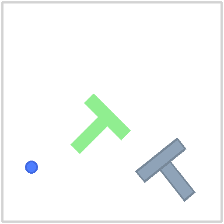
\includegraphics[width=1.10cm]{figures/split_assets/pusht_v0.png}};
 \else
  \node[inner sep=0pt] at (8.24,\yy) {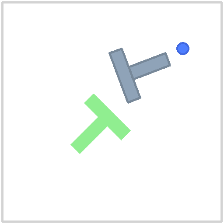
\includegraphics[width=1.10cm]{figures/assets/method_train_other.png}};
 \fi
 \node at (7.37,\yy) {$v_0$};
 \node[shell,draw=obsblue!50,minimum width=1.08cm,minimum height=.58cm] (ocmap\tag) at (10.02,\yy) {$C_o$};
 \draw[flow] (8.84,\yy) -- (ocmap\tag.west);
 \node[text=ink!65] at (9.15,\yy+.26) {$E_0$};
 \node[code,draw=obsblue,fill=obsblue!5] (oc\tag) at (11.71,\yy) {$c_o^{\tag}$};
 \draw[flow] (ocmap\tag.east) -- (oc\tag.west);
}
\draw[pair,draw=obsblue] (oci.south) -- (ocj.north);
\node[text=obsblue,font=\fontsize{12}{14}\selectfont] at (12.47,1.76) {$\mathcal L_o$};
\end{scope}
\end{tikzpicture}
}
\caption{\textbf{ShiftWM (ours): separate contexts with paired supervision.}
\textbf{A} infers observation context from past-feature statistics and shares
one calibration map between history and goal. \textbf{B} infers dynamics
context from corrected transitions and executed actions, then conditions
action embeddings in the reused LeWM predictor. \textbf{C} adds offline
penalties: $\mathcal L_d$ compares different appearances of the same trajectory
and actions, each through its own A--B computation; $\mathcal L_o$ compares
distinct batch entries with the same appearance. Dashed links denote penalties,
not guaranteed equal or identified contexts. Training frames in C represent
support clips; the upper frames illustrate deployment inputs. The encoder is
frozen; contexts, adapters, and reused prediction modules train offline.
Online, weights and contexts stay fixed within CEM search. Each candidate
action sequence produces a latent rollout, scored by terminal MSE to the
calibrated goal. CEM refits its action distribution to low-cost elites;
the controller executes the first block of the final mean plan and replans.
Feature glyphs and the rollout/cost example are schematic, not measurements.
Canonical query losses and the exact planning budget are given in the text.}
\label{fig:method}
\end{figure}

\subsubsection{Context inference and prediction}
For $u_t=E_0(o_t)\in\R^d$, the observation pathway computes
\begin{equation}
 c_o=C_o(u_S),\qquad z_t=A_o(u_t,c_o).
 \label{eq:obs}
\end{equation}
The residual adapter $A_o$ calibrates shifted features to reference
coordinates. Dynamics context uses chronological corrected support and
executed actions:
\begin{align}
 c_d&=C_d\big((z_i,a_i,z_{i+1})_{i\in S}\big),\nonumber\\
 \widetilde a_t&=A_d(E_a(a_t),c_d),\qquad
 \hat z_{t+1}=P_\theta(z_{t-L+1:t},\widetilde a_{t-L+1:t}).
 \label{eq:prediction}
\end{align}
Here $A_d$ is an action-embedding adapter and $L$ is predictor history.
Correcting support before dynamics inference is an inductive bias, not
proof of independence; uninformative actions can leave dynamics ambiguous.
Contexts are inferred once per replan and held fixed over candidate rollouts.

\subsubsection{Learning in fixed coordinates}
For a canonical training render $o_t^*=R_{v_0}(x_t)$, the target is
$z_t^*=\sg(E_0(o_t^*))$. The prediction loss $\mathcal L_{\mathrm{pred}}$
is teacher-forced one-step query MSE, and $\mathcal L_{\mathrm{align}}$
is corrected-feature MSE to the same frozen reference. Appearance variants
of the same trajectory encourage equal dynamics contexts through
$\mathcal L_d$. Different batch examples sharing an appearance label
encourage equal observation contexts through $\mathcal L_o$.
The objective is
\begin{equation}
 \mathcal L=\mathcal L_{\mathrm{pred}}
 +\lambda_{\mathrm{align}}\mathcal L_{\mathrm{align}}
 +\lambda_d\mathcal L_d+\lambda_o\mathcal L_o,
 \label{eq:loss}
\end{equation}
with weights $(1,0.1,0.01)$. Unpaired contexts disable the two consistency
terms. Targets have fixed coordinates, but the contexts themselves may
collapse or rescale with their adapters. Constant-context and shuffled-context
controls are therefore required before interpreting the contexts as useful
factor-specific information. Appendix~\ref{sec:loss-details} states the
exact index sets and batch-pairing rules, including the mismatch between
one-step training and recursive evaluation.

\subsubsection{Planning}
The goal embedding is $z_g=A_o(E_0(o_g),c_o)$, assuming the goal shares
the current observation setting. A common CEM/MPC solver minimizes
\begin{equation}
 J(a_{t:t+K-1})=\operatorname{mse}(\hat z_{t+K},z_g),
 \label{eq:cost}
\end{equation}
executes the first action chunk, and replans from new real observations.
All methods share candidate count, iterations, action bounds, horizon,
and paid interaction budget. Different-view goals and online gradient
adaptation are outside the completed primary comparison.

\subsection{Experiments}
\label{sec:experiments}
\paragraph{Tasks and composition.}
We use visual PushT and Reacher in \texttt{stable-worldmodel}. Appearance
factors are canonical, warm, and cool RGB transforms. PushT varies damping;
Reacher varies arm and finger density together. Seven factor pairs train the
model, $(v_1,p_1)$ is development, and $(v_2,p_2)$ is held-out composition
(Figure~\ref{fig:split}). Separate extrapolation tests introduce dim appearance
and a new physical value. Each environment has 256 training, 32 validation,
32 development, and 64 test initial-state seeds. Test trajectories are
independent and cover all nine in-range pairs; extrapolation covers three
additional pairs. Appendix~\ref{sec:protocol-details} gives exact values,
episode counts, and action interfaces.

\begin{figure}[t]
\centering
\resizebox{\linewidth}{!}{% Canonical editable geometry. Real training frames + exact pointwise RGB variants.
% Response arrows are schematic, not measured trajectories; see split_visual_brief.md.
\begingroup%
\definecolor{splitInk}{HTML}{233548}%
\definecolor{splitMuted}{HTML}{607389}%
\definecolor{splitLine}{HTML}{D5DEE7}%
\definecolor{splitPale}{HTML}{F4F7FA}%
\definecolor{splitBlue}{HTML}{0072B2}%
\definecolor{splitOrange}{HTML}{B75B16}%
\definecolor{splitViolet}{HTML}{7751A6}%
\begin{tikzpicture}[x=1cm,y=1cm,>=Latex,
  font=\sffamily\fontsize{9}{10}\selectfont,text=splitInk,
  heading/.style={font=\sffamily\bfseries\fontsize{10}{11}\selectfont},
  note/.style={font=\sffamily\fontsize{8}{9}\selectfont},
  actionarrow/.style={-{Latex[length=2.7pt,width=2.15pt]},splitBlue,line width=.65pt},
  responsearrow/.style={-{Latex[length=2.4pt,width=1.9pt]},splitOrange,line width=.60pt},
  pics/train/.style={code={\fill[splitMuted] (0,0) circle (.105);}},
  pics/dev/.style={code={\draw[splitOrange,fill=splitOrange!15,line width=1pt]
    (0,.18)--(.18,0)--(0,-.18)--(-.18,0)--cycle;}},
  pics/heldout/.style={code={\fill[splitBlue]
    (90:.27)--(54:.115)--(18:.27)--(-18:.115)--(-54:.27)--(-90:.115)
    --(-126:.27)--(-162:.115)--(-198:.27)--(-234:.115)--cycle;}},
  pics/extra/.style={code={\draw[splitViolet,fill=splitViolet!8,line width=1.1pt]
    (0,.21)--(.20,-.14)--(-.20,-.14)--cycle;}}]
\path[use as bounding box] (0,-.15) rectangle (13.97,7.35);

% Two identifiable observed task scenes, not successful-rollout examples.
\node[heading] at (1.34,6.98) {PushT};
\node[note,text=splitMuted] at (1.34,6.59) {damping};
\node[inner sep=0pt] at (1.34,5.02)
  {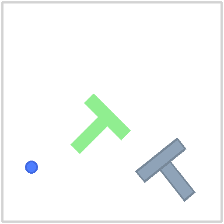
\includegraphics[width=2.55cm]{figures/split_assets/pusht.png}};
\node[heading] at (1.34,3.45) {Reacher};
\node[note,text=splitMuted] at (1.34,3.08) {density};
\node[inner sep=0pt] at (1.34,1.46)
  {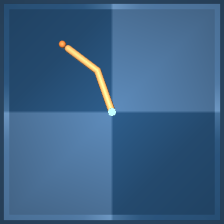
\includegraphics[width=2.55cm]{figures/split_assets/reacher.png}};

% One repeated observed state: only colors change between row headers.
\node[heading] at (4.11,6.98) {Appearance};
\node[note,text=splitMuted] at (4.11,6.59) {same state};
\foreach \row/\yy in {0/4.85,1/3.65,2/2.45,3/1.15}{
  \node[inner sep=0pt] at (4.15,\yy)
    {\includegraphics[width=1.08cm]{figures/split_assets/pusht_v\row.png}};
  \node[anchor=east] at (3.45,\yy) {$v_{\row}$};
}
\node[note,text=splitViolet] at (3.20,.80) {new};

% Same-input/different-response analogy. Lengths and rotations are non-quantitative.
\node[heading] at (9.30,6.98) {Dynamics};
\node[note,text=splitMuted] at (9.30,6.59) {same action; schematic responses};
\foreach \xx/\dx/\dy/\angle/\index in
  {6.35/.55/.03/10/0,8.35/.61/.13/-20/1,10.35/.55/.18/25/2,12.65/.63/.01/-10/3}{
  \begin{scope}[shift={(\xx,5.87)}]
    \fill[splitMuted] (-.61,-.06)--(-.30,-.06)--(-.30,.04)--(-.40,.04)
      --(-.40,.24)--(-.51,.24)--(-.51,.04)--(-.61,.04)--cycle;
    \fill[splitBlue] (-.80,-.10) circle (.059);
    \draw[actionarrow] (-.88,-.29)--(-.37,-.29);
    % Connector bounds are separated from both the initial and rotated response glyphs.
    \draw[responsearrow] (-.17,.04)--(.25,\dy+.03);
    \begin{scope}[shift={(\dx,\dy)},rotate=\angle]
      \draw[splitOrange,fill=splitOrange!18,line width=.65pt]
        (-.15,-.06)--(.15,-.06)--(.15,.04)--(.055,.04)
        --(.055,.24)--(-.055,.24)--(-.055,.04)--(-.15,.04)--cycle;
    \end{scope}
  \end{scope}
  \node at (\xx,5.35) {$p_{\index}$};
}
\node[note,text=splitViolet,anchor=west] at (12.93,5.35) {new};

% A quiet crossing map: positions carry the split, symbols carry membership.
\fill[splitPale,rounded corners=4pt] (5.42,1.88) rectangle (11.27,5.11);
\foreach \yy in {4.25,3.05}{\draw[white,line width=1pt] (5.42,\yy)--(11.27,\yy);}
\foreach \xx in {7.35,9.35}{\draw[white,line width=1pt] (\xx,1.88)--(\xx,5.11);}
\draw[splitViolet!65,densely dashed,line width=.75pt] (11.63,.62)--(11.63,6.02);
\draw[splitViolet!65,densely dashed,line width=.75pt] (3.57,1.80)--(13.65,1.80);
\foreach \xx/\yy in {6.35/4.85,8.35/4.85,10.35/4.85,6.35/3.65,10.35/3.65,6.35/2.45,8.35/2.45}{
  \pic at (\xx,\yy) {train};
}
\pic at (8.35,3.65) {dev};
\pic at (10.35,2.45) {heldout};
\foreach \xx/\yy in {12.65/4.85,6.35/1.15,12.65/1.15}{\pic at (\xx,\yy) {extra};}

% One legend; no repeated prose in cells. Blank intersections are untested.
\pic at (4.06,.20) {train};
\node[note,anchor=west] at (4.31,.20) {Train (7)};
\pic at (6.07,.20) {dev};
\node[note,anchor=west] at (6.36,.20) {Dev.};
\pic[scale=.70] at (7.68,.20) {heldout};
\node[note,anchor=west] at (7.96,.20) {Held-out pair};
\pic at (10.70,.20) {extra};
\node[note,anchor=west] at (11.02,.20) {Extrapolation};
\end{tikzpicture}%
\endgroup%
}
\caption{\textbf{Composition protocol.} Real task frames and exact RGB transforms
illustrate observation changes; response glyphs are schematic. PushT varies
damping and Reacher varies density. Seven pairs train the model, $(v_1,p_1)$
is development, and $(v_2,p_2)$ is held-out composition. Three extrapolation
pairs introduce new values. Independent test trajectories cover all nine
in-range pairs. Split identities precede paired rendering; factor labels are
unavailable to the deployed model.}
\label{fig:split}
\end{figure}

\paragraph{Compared methods.}
\emph{Frozen LeWM} is the released pretrained reference. \emph{Framewise
calibration}, \emph{Shared context}, and \emph{Unpaired contexts} are our
matched controls on that same backbone, not independent reproductions of
published methods (Table~\ref{tab:methods}). Framewise calibration tests
whether per-image correction suffices. Shared context tests whether one
inferred context is sufficient. Unpaired contexts retains the two-branch
architecture while removing context-consistency losses. \emph{ShiftWM
(ours)} combines separate contexts with those paired losses. Every trained
variant has three seeds and 30 completed epochs; ordinary-validation
prediction error selects checkpoints. The \emph{Unaligned predictor}
retains mismatched observed/goal coordinates and is reported only as a
diagnostic in Appendix~\ref{sec:full-results}.

\IfFileExists{generated/method_comparison.tex}{
\begin{table}[t]
\centering\small
\caption{\textbf{Methods in the primary comparison.} Frozen LeWM is the
released reference; the other rows are matched in-house implementations on
its backbone. Every learned visual calibration path uses canonical alignment.
Only ShiftWM uses paired context consistency. None uses online gradients.}
\label{tab:methods}
% Sources: src/shiftwm/model.py and configs/world/*_s0.json.
\begingroup\small\setlength{\tabcolsep}{5pt}\renewcommand{\arraystretch}{1.12}
\begin{tabular}{@{}llll@{}}\toprule
Method & Visual calibration & Context & Consistency\\\midrule
Frozen LeWM & None & None & None\\
Framewise calibration & Per frame & None & None\\
Shared context & Contextual & Shared & None\\
Unpaired contexts & Contextual & Separate & None\\
\textbf{ShiftWM (ours)} & Contextual & Separate & Paired\\
\bottomrule\end{tabular}\endgroup

\end{table}
}{}

\paragraph{Metrics and evaluation budget.}
Closed-loop success is primary. The main comparison separates the held-out
pair from extrapolation; canonical and all-condition results remain in the
appendix. Planning uses 300 CEM candidates, 30 iterations, 30 elites, a
five-group horizon, and five native controls per group. The 50-native-step
budget includes ten support-acquisition steps. Methods use matched
initial-state/goal identities and common support. Raw success includes
support-only successes; policy-eligible success excludes them. Table entries
require all three trained seeds and report mean $\pm$ sample standard
deviation, while paired task-cluster intervals appear separately in
Appendix~\ref{sec:paired-planning}. Forecast MSE@5 uses five recursive
transitions with recorded actions in immutable reference coordinates.
Hyperparameters are fixed without test-based selection; elapsed inference
time is not compared without dedicated hardware measurements.

\subsection{Results and analysis}
\label{sec:results}
All 30 training runs, main forecast evaluations, and 64 prescribed
checkpoint--split planning evaluations are complete.
Table~\ref{tab:measured-primary} is the main closed-loop comparison; every
trained-method entry now includes all three prescribed seeds and passes
source and protocol validation. Full
condition results, eligibility counts, and exact forecast values are in
Appendix~\ref{sec:full-results}.

\IfFileExists{generated/primary_results.tex}{
% Generated primary planning comparison; diagnostics are reported separately.
\begin{table}[t]\centering\small
\providecommand{\ShiftWMPlanningGainRows}{}
\InputIfFileExists{generated/planning_gain_rows.tex}{}{}
\setlength{\tabcolsep}{5pt}\renewcommand{\arraystretch}{1.12}
\begin{tabular}{lrrrr}\toprule
& \multicolumn{2}{c}{PushT} & \multicolumn{2}{c}{Reacher}\\
\cmidrule(lr){2-3}\cmidrule(l){4-5}
Method & Held-out $\uparrow$ & Extrap. $\uparrow$ & Held-out $\uparrow$ & Extrap. $\uparrow$\\\midrule
Frozen LeWM & 4.7 & 7.3 & 35.9 & 17.7\\
Framewise calibration & 3.6 $\pm$ 0.9 & 5.0 $\pm$ 0.8 & 42.7 $\pm$ 3.3 & 21.2 $\pm$ 5.9\\
Shared context & 2.1 $\pm$ 0.9 & 7.6 $\pm$ 1.1 & 36.5 $\pm$ 3.9 & 16.8 $\pm$ 3.3\\
Unpaired contexts & 2.6 $\pm$ 0.9 & 5.2 $\pm$ 1.4 & 34.9 $\pm$ 9.0 & 20.8 $\pm$ 2.6\\
\addlinespace[2pt]
\rowcolor{orange!9}
\textbf{ShiftWM (ours)} & 2.6 $\pm$ 0.9 & 6.8 $\pm$ 0.5 & 40.6 $\pm$ 3.1 & 19.6 $\pm$ 1.3\\
\ShiftWMPlanningGainRows
\bottomrule\end{tabular}
\caption{\textbf{Main comparison: closed-loop planning success (\%).} Higher is better. Trained entries require all three seeds and show mean $\pm$ sample SD; Frozen LeWM uses one released checkpoint per environment. The final rows give ShiftWM minus Shared context in percentage points and conditional 95\% paired task-cluster intervals, not SD. \positivegain{Bold green} marks positive mean differences, not statistical significance. Dashes denote incomplete evidence, not zero success. Held-out is $(v_2,p_2)$; extrapolation averages three prespecified conditions. All methods share the paid support and planning budget. Framewise calibration, Shared context and Unpaired contexts are in-house controls on the same LeWM backbone. Full metrics and the unaligned diagnostic appear in Table~\ref{tab:measured-full}.}
\label{tab:measured-primary}\label{tab:primary}\end{table}

}{\draftnote{Primary comparison tables await generated evidence records.}}

\paragraph{Does composition improve planning?}
The complete matched comparisons show mixed effects. Relative to Framewise
calibration, held-out raw-success differences are $-1.04$ percentage points
on PushT (conditional 95\% interval $[-3.65,1.56]$) and $-2.08$ on Reacher
($[-11.46,7.29]$). On extrapolation, PushT improves by $+1.74$ points
($[0.00,3.65]$), while Reacher declines by $-1.56$ ($[-6.25,3.13]$).
These intervals condition on the three observed training seeds.

Positive held-out point estimates occur against Shared context ($+0.52$
points on PushT and $+4.17$ on Reacher) and against Unpaired contexts on
Reacher ($+5.73$); PushT ties Unpaired contexts. Across the 12 raw-success
contrasts in Table~\ref{tab:paired-planning}, six means are positive, five
negative, and one zero. Every conditional 95\% interval includes zero;
the PushT extrapolation interval against Framewise touches it exactly.
The intervals are not multiplicity-adjusted and do not capture uncertainty
over the population of training runs. The completed evidence therefore
does not establish consistent planning superiority or isolate a benefit
from context pairing. Policy-eligible comparisons, with support-only
successes excluded, are reported alongside the raw contrasts.
\IfFileExists{generated/primary_comparison_status.tex}{
All prescribed three-seed planning comparisons with Framewise calibration and Unpaired contexts are available in Table~\ref{tab:measured-primary}, with paired uncertainty reported in Table~\ref{tab:paired-planning}.

}{Their completion status is given in Table~\ref{tab:measured-primary}.}
Differences only against Frozen LeWM would conflate the proposed structure
with additional training.

\paragraph{Where ShiftWM improves forecasting.}
Against the fixed Framewise calibration reference, ShiftWM achieves
\textbf{26.78\% lower held-out Reacher MSE@5} and 3.68\% lower PushT MSE@5,
using ratios of three-seed means (Figure~\ref{fig:results}). The closest
aligned held-out comparator is Unpaired contexts: adding paired consistency
reduces its error by 9.21\% on Reacher and 2.30\% on PushT. These are
relative forecast-error reductions, not changes in planning success.
\IfFileExists{generated/forecast_gain_summary.tex}{
\begin{center}
\small
% Positive relative reduction means lower MSE; negative means regression.
\begingroup\small\setlength{\tabcolsep}{5pt}\renewcommand{\arraystretch}{1.1}
\begin{tabular}{@{}lrrrr@{}}
\multicolumn{5}{@{}l}{\textbf{Relative MSE reduction (\%) $\uparrow$}}\\[3pt]\toprule
& \multicolumn{2}{c}{PushT} & \multicolumn{2}{c}{Reacher}\\
\cmidrule(lr){2-3}\cmidrule(l){4-5}
Reference & Held-out & Extrap. & Held-out & Extrap.\\\midrule
Framewise calibration & \positivegain{+3.68} & \positivegain{+4.20} & \positivegain{+26.78} & -4.15\\
Unpaired contexts & \positivegain{+2.30} & \positivegain{+0.70} & \positivegain{+9.21} & -0.35\\
\bottomrule\end{tabular}\endgroup

\end{center}
}{}
The summary defines reduction as $100(\mathrm{baseline}-\mathrm{ours})/
\mathrm{baseline}$, so positive means lower error and negative means a
regression. \positivegain{Bold green} marks positive mean reductions, not
statistical significance. On extrapolation, PushT improves over Framewise calibration by
4.20\%, while Reacher worsens by 4.15\%; Frozen LeWM has the lowest
Reacher extrapolation error among the aligned models. The unaligned
diagnostic has lower held-out PushT error than ShiftWM and remains visible
in the full results. Thus, the held-out gains do not establish uniform
superiority. Unpaired contexts also improves on Shared context in both
held-out environments, separating architectural changes from pairing.
Mean ordering and three-seed dispersion do not identify the factors encoded
by either context or constitute a significance test.

\IfFileExists{generated/forecast_comparison.pdf}{
\begin{figure}[H]
\centering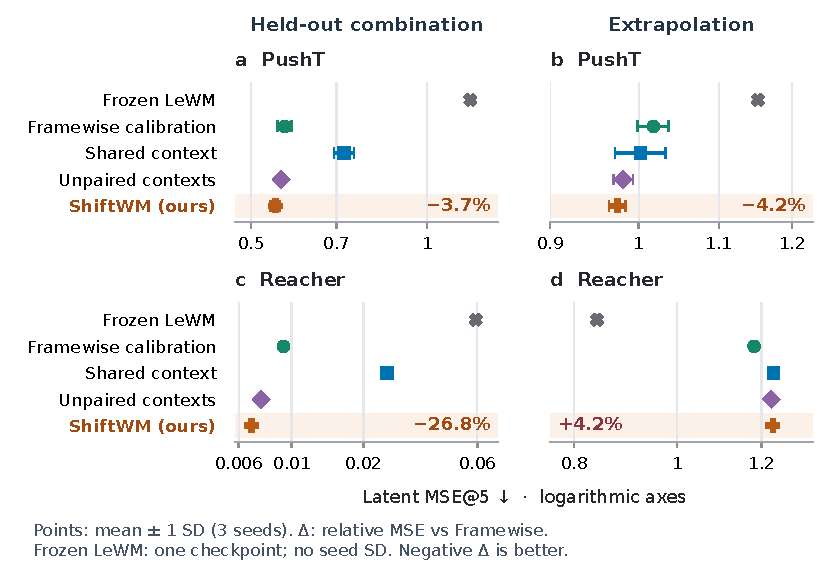
\includegraphics[width=\linewidth]{generated/forecast_comparison.pdf}
\caption{\textbf{Forecasting on held-out composition and extrapolation.}
Terminal latent MSE after five recursive transitions (25 native actions)
using recorded future actions; lower is better. Points and ranges show
three-training-seed means and sample standard deviations, not confidence
intervals. Frozen LeWM has one checkpoint and no training-seed error bar.
Extrapolation averages the three prespecified new-value conditions. Horizontal
axes are logarithmic with panel-specific limits; latent coordinates differ by
environment. Gain annotations use signed error change relative to Framewise
calibration: negative means lower MSE. These ratios of three-seed means are
point summaries, not significance estimates. Forecast accuracy alone does
not establish planning success.}
\label{fig:results}
\end{figure}
}{\draftnote{The forecast plot awaits complete source-validated records.}}

\paragraph{Why better forecasts need not yield better control.}
In the completed seed-0 development comparison, ShiftWM and Shared context
have equal success rates; Framewise calibration has the highest Reacher
point estimate. A subsequent goal-only intervention keeps the ShiftWM
predictor fixed but substitutes framewise goal correction. Eligible Reacher
success increases from 6/30 to 12/30, compared with 11/30 for the complete
framewise controller; PushT falls from 1/31 to 0/31
(Appendix~\ref{sec:goal-calibration}). This post-hoc intervention motivates
separate checks of prediction and goal alignment, not a general repair.
CEM also selects its own candidate actions, so mean forecast error on
recorded trajectories does not control error on those selected candidates.
Mechanism tests, the completed dynamics-residual revision, and the completed
controlled rollout-objective study are described in
Appendices~\ref{sec:mechanism}, \ref{sec:dynamics-revision}, and
\ref{sec:rollout-revision}.
Matched observed rollouts in Appendix~\ref{sec:qualitative-rollouts}
show successes, failures, and goals reached during support before planning.



